% Section des résultat: Application sur des réseaux biologiques

In this section, we exhibit several experiments conducted on biological networks.
We detail the results or our implementation
on a 4-components model of the lambda phage,
and recapitulate the results and performance of some benchmarks
on other models up to 28 components.
In general, the time performances are good and
the overall results seem to support the use of ASP for the verification
of formal properties or the enumeration of special constructs
on biological systems.

All experiments were run on a desktop PC
with a Pentium VII 3 GHz processor and 16 GB memory.

\subsection{Lambda phage model}
\begin{figure}[h]
  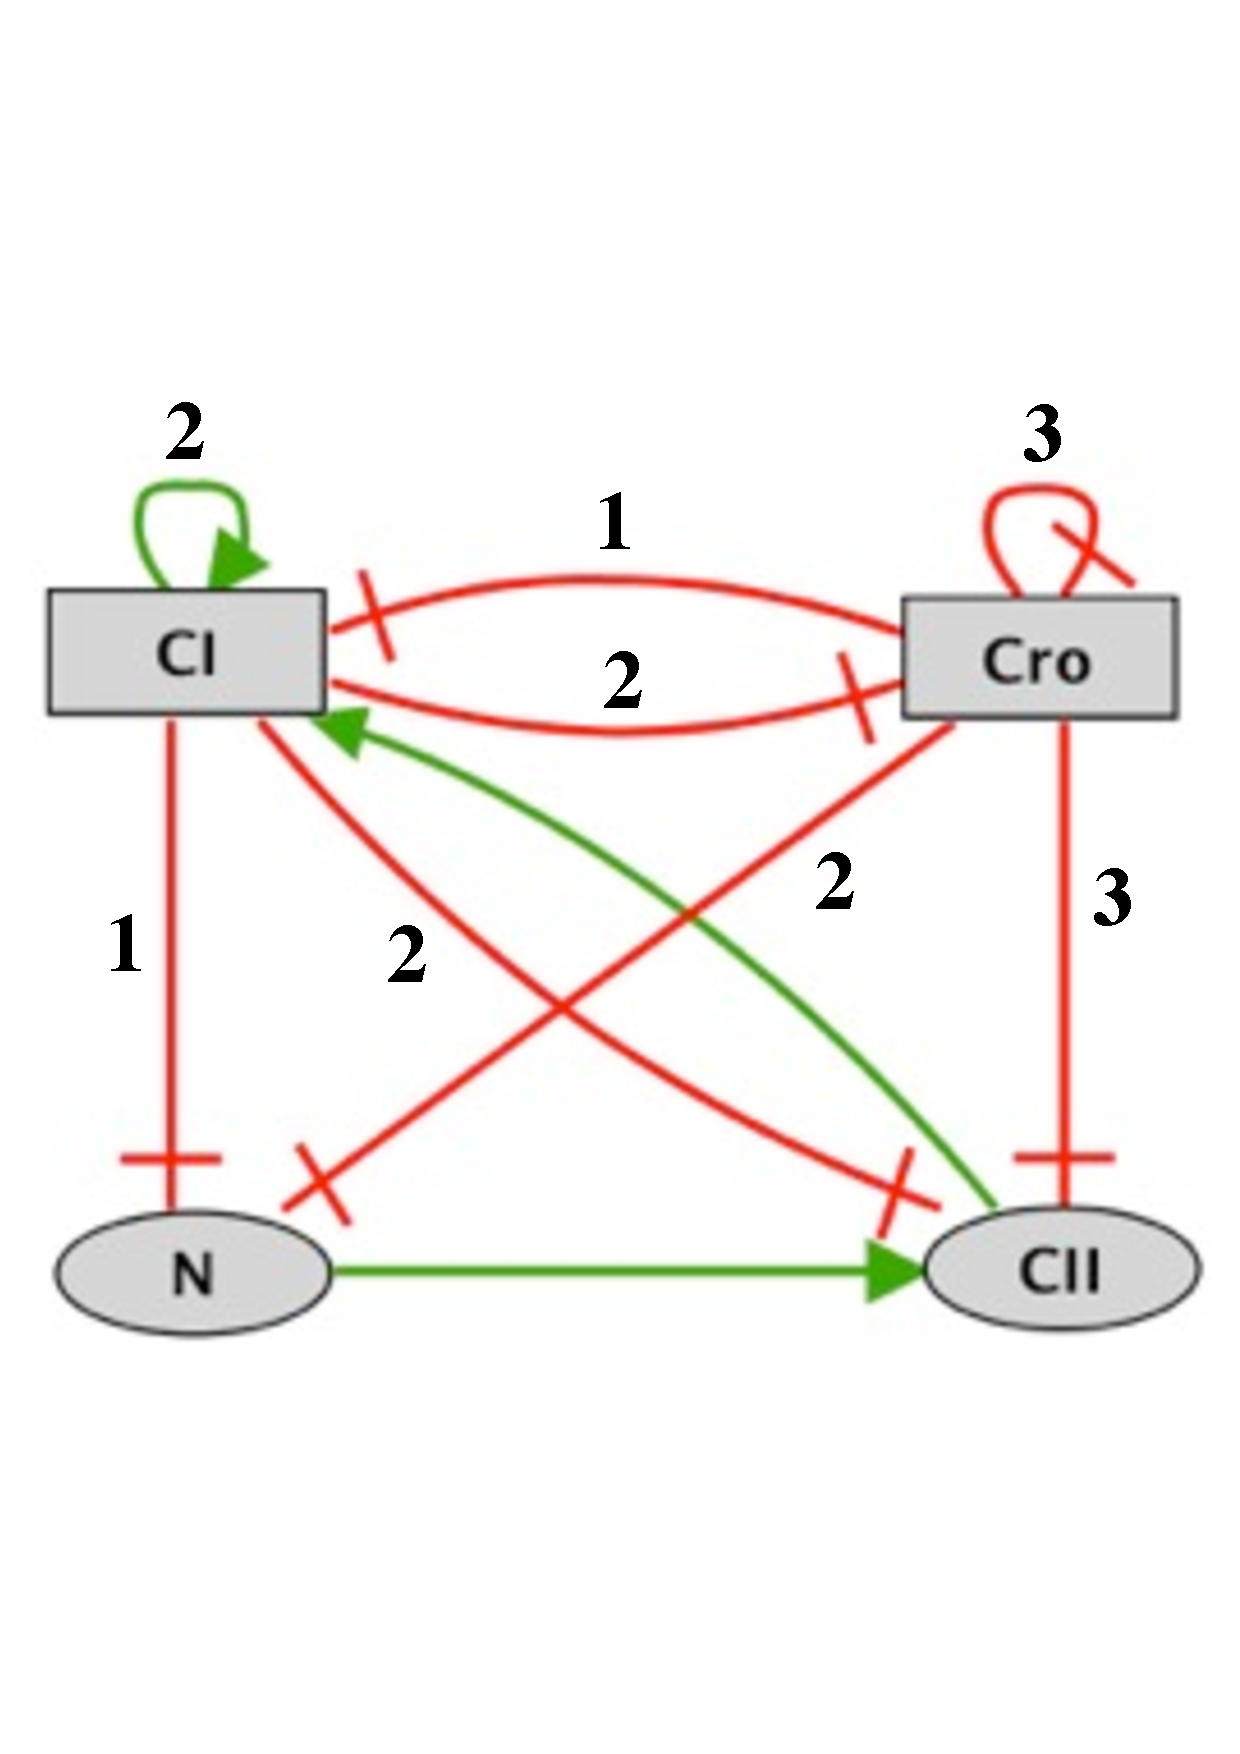
\includegraphics{figures/lampdaphage-thomas.pdf}
  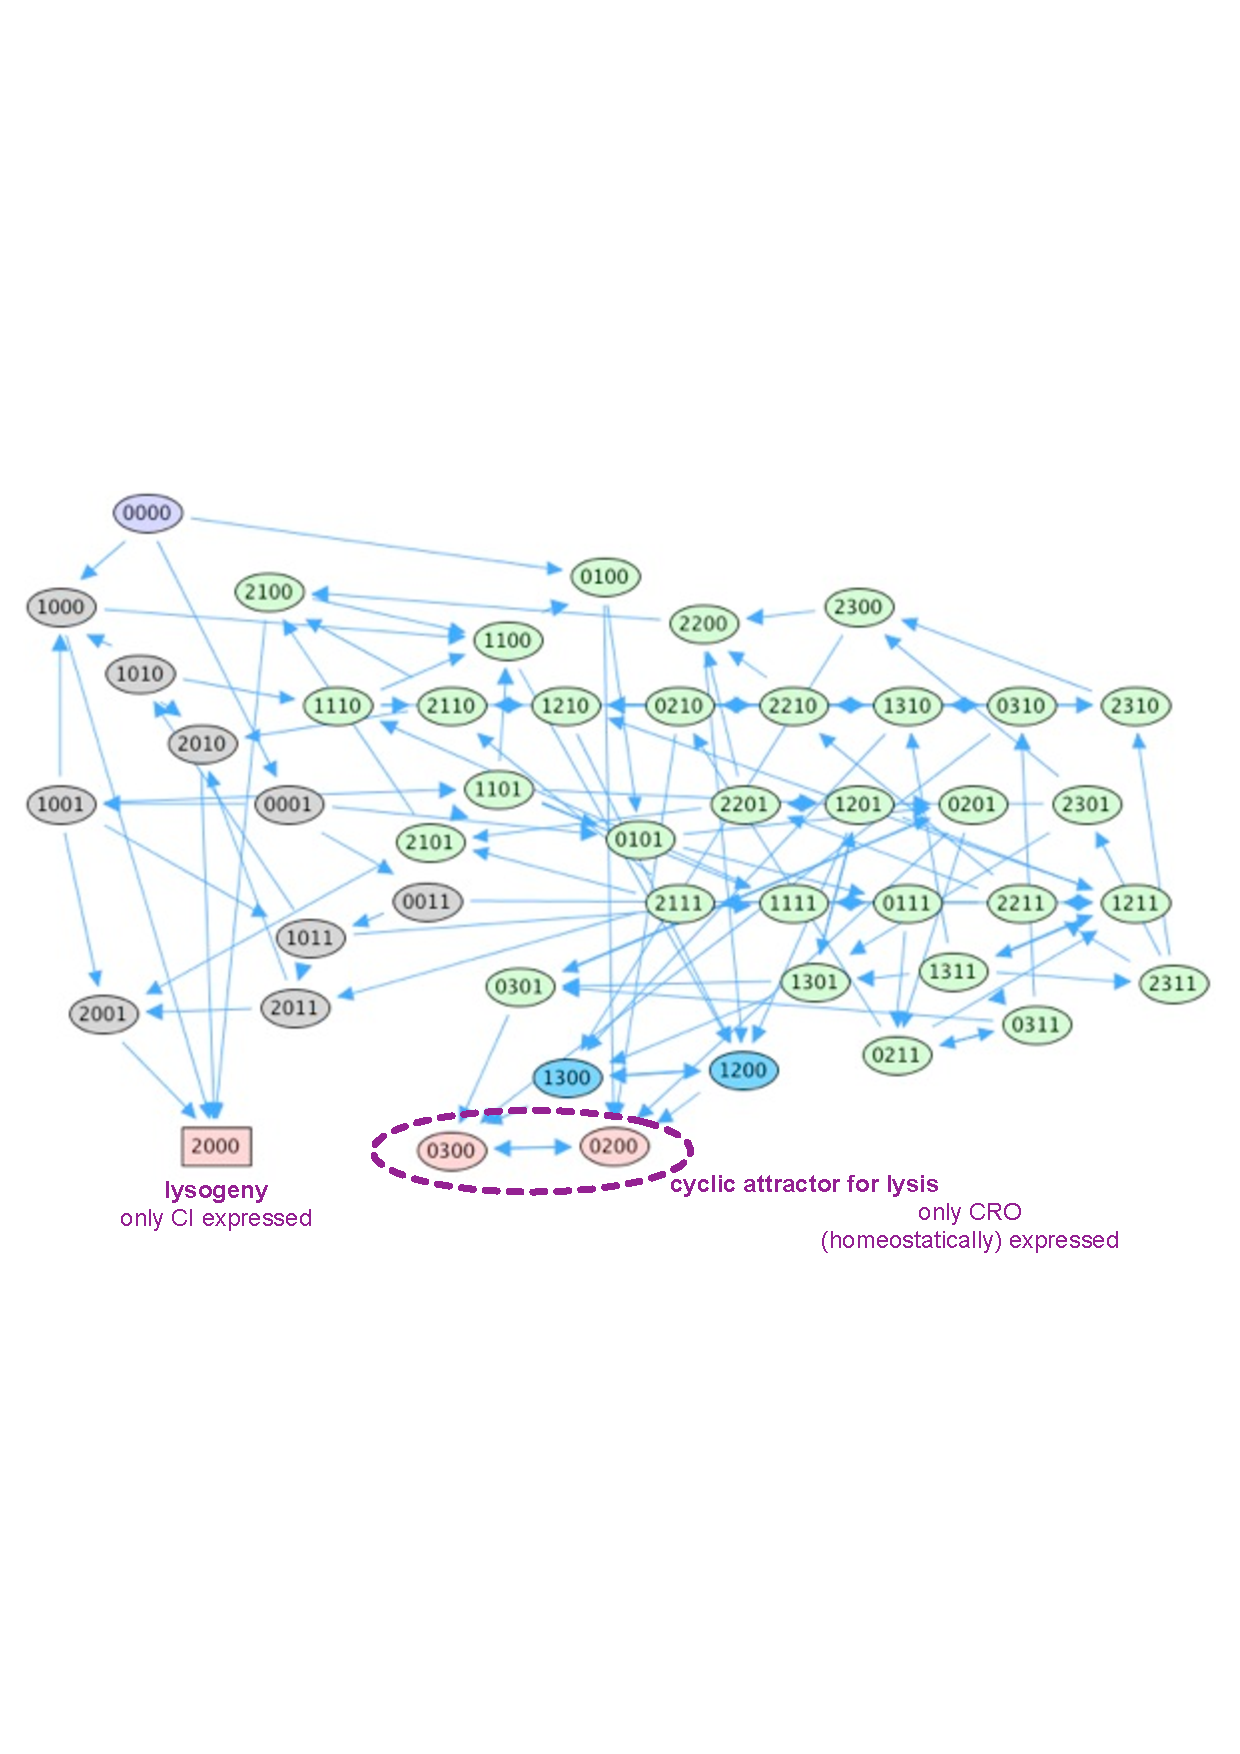
\includegraphics{figures/lampdaphage-STG.pdf}
  \caption{\label{fig:lambda-graph} 
    Descriptions of the 4-components lambda phage model used for our experiments.
    The left figure presents the regulatory graph used with positive and negative regulations represented by ’$+$’ and ’$-$’ symbols.
    The right figure is the corresponding state transition graph (STG).% colored according to strongly connected components. 
    We can observe two attractors: $(2000)$ is an attractor of size $1$, \ie a fixed point and $\{(0300), (0200)\}$ is an attractor of size $2$.
    Figures were taken from \cite{thieffry1995dynamical,chaouiya2008petri}.
  }
\end{figure}

We first conducted detailed experiments on a 4-components model of the bacteriophage lambda system described in \pref{fig:lambda-graph} \cite{thieffry1995dynamical}.
This network was modeled as a PH network containing 4 sorts, 48 processes and 49 actions.
Its State-Transition Graph (STG) comprises \Emna{???} different states.

An analytic study of the minimal trap domains on this small network
allows to find the following structures:
\begin{itemize}
  \item exactly one fixed point: $\PHstate{CI_2, CII_0, Cro_0, N_0}$
  \item exactly one cyclic attractor: $\{ \PHstate{CI_0, CII_0, Cro_2, N_0}$, $\PHstate{CI_0, CII_0, Cro_3, N_0} \}$
\end{itemize}
We note that the attractor happens to be of size 2.

The implementation of the method described in \pref{sec:fixpoint} and \pref{sec:attractors}
of course returns the same results.
The output of the fixed points enumeration program is straightforward,
as it contains exactly one answer set (corresponding to the only existing fixed point) which describes the only stable state of the model:
\begin{lstlisting}[numbers=none]
Answer: 1
selectProc("CI",2) selectProc("CII",0)
selectProc("Cro",0) selectProc("N",0)
\end{lstlisting}
Performing the search for size-2 attractors also returns exactly one answer set corresponding to the only attractor of that size.
In the output, each state belonging to this attractor is labeled by a number (\texttt{0} and \texttt{1}) allowing to enumerate all active processes in both states:
\begin{lstlisting}[numbers=none]
Answer: 1
selectProcSt(activeProc("CI",0),0) selectProcSt(activeProc("CII",0),0)
selectProcSt(activeProc("Cro",2),0) selectProcSt(activeProc("N",0),0) 
selectProcSt(activeProc("CI",0),1) selectProcSt(activeProc("CII",0),1)
selectProcSt(activeProc("Cro",3),1) selectProcSt(activeProc("N",0),1)
\end{lstlisting}
Moreover, executing out implementation for $N>2$ returns no results,
which is expected because there exists no attractor of size strictly bigger than two, and we excluded repeated loops from the results (therefore the already found size-2 attractor is not found for $N=4$).
On this small network, all results are computed in less than a tenth of a second.

\subsection{Benchmarks}
In the following, we propose some additional benchmarks to demonstrate
the capabilities of our implementation.
We do not give the detail of the results of these experiments
but rather focus on the size of the outputs and the computation times.
We used several preexisting multi-valued networks inspired from real organisms
and found in the literature:
a bacteriophage lambda \cite{thieffry1995dynamical},
a hedgehog signaling pathway (\Emna{à revoir la réf} \cite{stecca2010context}),
an mTOR pathway in survival mechanisms \cite{javle2010inhibition} (\Emna{en cours de traduction})
and a mammalian signaling pathway induced by the Epidermal Growth Factor (EGF) and Tumour Necrosis Factor alpha (TNF$\alpha$) \cite{chaouiya2013sbml}.
The ASP description of these networks in PH form has been realized manually
from the data given in the corresponding papers.
Results of these benchmarks\benchmarksfootnote{} are given in \pref{tab:models}.

\begin{table*}[ht]
\begin{center}
\noindent%
%\begin{tabular}{| l| c | c | c ||>{\columncolor{verylightgray}} c | c ||>{\columncolor{verylightgray}}c | c | c ||}
\begin{tabular}{| l || c | c | c || c | c || c | c | c |}
\hline
  \multicolumn{1}{| l ||}{\textbf{Models}} &
    \multicolumn{3}{c||}{\textbf{PH model}} &
    \multicolumn{2}{c||}{\textbf{Fixed points}} &
    \multicolumn{3}{c|}{\textbf{Attractors}}\\
\hline
  &
%    sorts & processes & states &
    $\card{\PHs}$ & $\card{\bigcup_a \PHl_a}$ & $\card{\PHl}$ &
    $\Delta t$ (s) & \#results &
    $N$ & $\Delta t$ (s) & \#results \\
\hline
\hline
%  TTR  & 12 & 42  & $2^{19}$ & 0.004 & 0 & 0.004 & k & 0\\
%\hline
%  ERBB & 42 & 152 & $2^{70}$ & 0.017 & 3 & 0.004 & k & 0\\
%\hline
%  TCR & 54 & 156 & $2^{73}$ & 0.021 & 1 & 0.004 & k & 0\\
%\hline  
  \multirow{3}{*}{\begin{minipage}{4em}\textbf{lambda phage}\end{minipage}} &
    \multirow{3}{*}{4} & \multirow{3}{*}{11} & \multirow{3}{*}{48} &
    \multirow{3}{*}{0.003} & \multirow{3}{*}{1} &
    2 & 0.019 & 1\\
    & & & & & & 4 & 0.033 & 0\\
    & & & & & & 20 & 0.470 & 0\\

\hline
  \multirow{3}{*}{\textbf{hedgehog}} &
    \multirow{3}{*}{5} & \multirow{3}{*}{11} & \multirow{3}{*}{48} &
    \multirow{3}{*}{0.003} & \multirow{3}{*}{2} &
    2 & 0.017 & 0\\
    & & & & & & 6 & 0.050 & 0\\
    & & & & & & 20 & 0.319 & 0\\

\hline
  \multirow{3}{*}{\textbf{mTOR}} &
    \multirow{3}{*}{6} & \multirow{3}{*}{12} & \multirow{3}{*}{$2^6$} &
    \multirow{3}{*}{0.009} & \multirow{3}{*}{1} &
    2 & 0.019 & 0\\
    & & & & & & 8 & 0.101 & 0\\
    & & & & & & 16 & 0.397s & 0\\

\hline
  \multirow{2}{*}{\textbf{egf-tnf}} &
    \multirow{2}{*}{28} & \multirow{2}{*}{56} & \multirow{2}{*}{$2^{28}$} &
    \multirow{2}{*}{0.005} & \multirow{2}{*}{2} &
    2 & 0 \Maxime{???!!!} & 0\\
    & & & & & & 8 & 9.192 & 1\\
% & & & & & & xxx & xx & x\\
\hline
\end{tabular}
\Maxime{--- Je pense qu'il vaudrait vraiment mieux donner le temps total pour trouver l'ensemble des attracteurs (on fait bien noter papier sur l'énumération). On peut donner les deux temps (énumération complète et premier attracteur trouvé).}

\Maxime{--- On peut encore gagner de la place horizontalement en insérant les résultats des points fixes en haut de ceux des attracteurs.}

\vspace*{4pt}
\caption{\label{tab:models}%
  Brief description of the models used in our benchmarks
  and the results of our fixed points and attractors enumerations.
  The successive lines sum up the information regarding, respectively,
  the bacteriophage lambda \cite{thieffry1995dynamical},
  the hedgehog signaling pathway \cite{stecca2010context},
  the survival mechanisms pathway (mTOR) \cite{javle2010inhibition}
  and the EGF- and TNF$\alpha$-induced mammalian signaling pathway (egf-tnf) \cite{chaouiya2013sbml}.
  For each of them, this table gives
  %the number of biological components in the original representation,
  the number of sorts and processes in the PH representation,
  and the number of states in the corresponding STG;
  the computation time and number of results of the fixed points enumeration;
  the computation time and number of results of the attractors enumeration for several sizes ($N$).
}
\end{center}
\end{table*}
